\part{Mantendo Suas Moedas Seguras}
\label{ch:capitulo6}
\chapter*{Mantendo Suas Moedas Seguras}

Até agora, falamos como gerenciamos e mantemos as cópias e gravamos no livro razão distribuído sem que possa haver coerção ou corrupção. Mas o que acontece quando um ganhador da loteria quer ser malicioso? Ganhar o direito de escrever em livro-razão significa que eles podem alterar lançamentos históricos no livro-razão? Evandro, Danilo e Fernanda podem conspirar para reescrever a história ou alterar os saldos das contas e dar a si mesmos moedas extras?

Vamos entrar na blockchain. Um termo de marketing que permeou grande parte do setor de tecnologia, a blockchain nada mais é do que a ideia de que os blocos do Bitcoin são encadeados para fornecer links de um conjunto de transações para o próximo bloco.

Mentimos um pouco no capítulo anterior para manter as coisas mais simples. Quando você minera jogando na loteria de Prova de Trabalho, você não está apenas fazendo o hash das transações que querem ir para o próximo bloco junto com o nonce. Na verdade, você também está fornecendo o hash do último bloco como entrada em sua função hash, vinculando assim seu bloco ao bloco anterior.

Isso nos permite construir um registro histórico de cada bloco desde o Bloco Gênesis (primeiro bloco do Bitcoin) extraído por Satoshi. Quando escrevemos um novo bloco na blockchain, temos que validar que este bloco não contém nenhuma transação que gaste bitcoins que já foram gastos em blocos anteriores.

\newpage

\begin{figure}
  \centering
  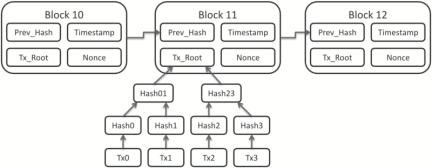
\includegraphics[width=10cm]{imagens/capitulo-06-bloco.jpg}
  \caption{\url{https://upload.wikimedia.org/wikipedia/commons/7/7a/Bitcoin_Block_Data.png}}
\end{figure}

Lembre-se de que a saída de uma função hash é aleatória e dependente de todos os dados de entrada que nela constam. Agora modificamos nossos hashes do bloco para incluir três entradas diferentes:

\begin{samepage}
\begin{enumerate}
\item As transações que queremos incluir no livro-razão;
\item Um nonce aleatório;
\item O hash do bloco anterior que estamos usando como sendo a base do histórico do livro-razão.
\end{enumerate}
\end{samepage}

Se alguma dessas três coisas forem alteradas, o hash de saída mudará de maneira imprevisível. Esse comportamento cria uma propriedade interessante: se você adulterar os dados de qualquer bloco antigo, alterará seu hash. Se você alterar o hash de qualquer bloco antigo, alterará o hash de cada bloco que vier depois.

Isso torna a corrente inviolável. Se alguém tentasse alterar um bloco mais antigo na cadeia, teria que recalcular o hash de Prova de Trabalho do bloco que está adulterando e de cada novo bloco que vier depois.

Efetivamente, cada novo bloco extraído no Bitcoin aumenta a segurança dos blocos que vieram antes dele. Uma transação em um bloco que possui 6 blocos posteriores a ele é considerada definitivamente inalterada. Seria necessária uma enorme quantidade de energia para recalcular os últimos seis blocos na taxa de hash total atual. Alterar um bloco a 100 blocos atrás? Nem pense nisso, esquece.

É importante entender que não há finalidade real de transação no Bitcoin. Cada comerciante ou processador de pagamentos decide por si mesmo o que considera final. Hoje, a maioria das pessoas aceita 6 confirmações - seis blocos extraídos depois daquele que contém a transação - como sendo definitivo, mas os comerciantes podem definir isso como quiserem.

Se você está vendendo um livro digital que tem custo marginal para você como comerciante, pode querer apenas 1 confirmação, ou mesmo zero confirmações, entregando o bem digital assim que vir a transmissão da transação na rede. Se você está vendendo uma casa, talvez queira esperar por doze confirmações, ou cerca de duas horas de mineração. Quanto mais você espera, mais Provas de Trabalho são empilhadas no topo do bloco que contém suas transações e mais caro se torna no mundo real para reverter a transação.

Se a taxa de hash do Bitcoin cair significativamente, o que significa que menos energia está protegendo cada bloco, pode-se sempre aumentar o número de confirmações necessárias para a liquidação final. Embora isso possa parecer muito complicado no início, é importante ter em mente que as transações com cartão de crédito normalmente podem ser revertidas 120 dias após serem feitas. Por outro lado, o Bitcoin é um dinheiro de liquidação final que não pode ser retirado de você, como dinheiro ou ouro. Deste ponto de vista, a reversibilidade e a finalidade das transações no Bitcoin é, na verdade, uma grande melhoria em relação à maioria das redes de pagamento tradicionais.

Vamos voltar ao nosso exemplo do Capítulo 3, onde Henrique se junta a uma rede e obtém diferentes cópias do livro-razão. O livro-razão que ele pegou da Carol é honesto, mas os livros-razão do Evandro, Danilo e Fernanda são maliciosos, onde eles excluíram um bloco antigo que continha os gastos originais da Alice para que eles pudessem enganar Henrique fazendo-o pensar que ela ainda tinha suas moedas. Antes de vincular os blocos entre si por Prova de Trabalho, Henrique não sabia que um bloco antigo foi excluído.

Como cada bloco contém uma Prova de Trabalho, ele sabe aproximadamente quanta energia foi consumida para produzi-lo com base no Número Alvo. Como cada bloco aponta para um bloco anterior, ele sabe que para alterar o histórico de um bloco antigo seria necessário recalcular a Prova de Trabalho não apenas do bloco adulterado, mas de cada bloco que veio depois dele. Como ele pode ver todas as transações em cada bloco, ele pode garantir que nenhum gasto duplo foi feito.

\begin{figure}
  \centering
  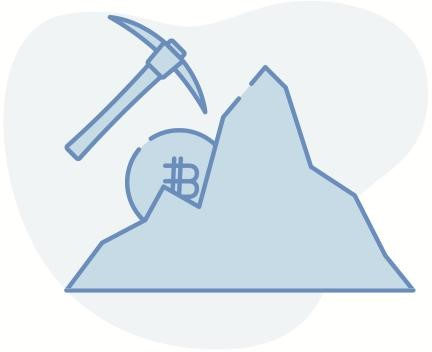
\includegraphics[width=5cm]{imagens/capitulo-06-mineracao.jpg}
  \caption{Ao contrário da mineração de ouro, que também consome energia, o processo de mineração de Bitcoin na verdade protege a rede para tornar o livro-razão à prova de adulteração.}
\end{figure}

\paragraph{E se duas pessoas encontrarem um bloqueio ao mesmo tempo?}
\paragraph{}

Falta uma peça no sistema de consenso. Imagine que agora estamos administrando uma rede mundial. Pessoas em todo o mundo, dos Brasil ao Japão, estão conectadas a essa rede global e todas estão jogando na loteria da Prova de Trabalho.

Alguém em São Paulo encontra um bloco válido. Eles o anunciam na rede e todos os computadores do Brasil começam a detectá-lo. Enquanto isso, alguém em Tókio também encontra um bloco a poucos segundos depois do bloco de São Paulo. Seus vizinhos ainda não ouviram falar do bloco brasileiro, então eles ficam sabendo primeiramente do bloco japonês.

Como os dois blocos se propagam através dos nodes vizinhos na rede, agora temos duas versões concorrentes da blockchain. Os brasileiros têm um que tem o bloco brasileiro no final, e os japoneses têm o seu próprio bloco. A rede está dividida por não saber qual a blockchain é a cópia correta do livro-razão, uma vez que ambos contêm quantidades equivalentes de Prova de Trabalho e ambos contêm transações válidas.

Você não pode contar com nenhum ente central para lhe dizer qual deles é o verdadeiro. O que você faz? O Bitcoin fornece uma solução bem simples para este problema: vamos apenas esperar para ver o que acontece. Existem agora duas versões concorrentes da blockchain. No próximo período de aproximadamente dez minutos, outro bloco será minerado. Os brasileiros estarão minerando no topo do bloco de que ouviram falar pela primeira vez, e os japoneses estarão minerando no topo de seu bloco.

Qualquer que seja o lado que minere primeiro, será o escolhido como sendo o verdadeiro. Como? Porque no código do Bitcoin há uma regra que diz que a cadeia de Prova de Trabalho Cumulativa Mais Longa resolve qualquer divisão que ocorra na cadeia. Quem consome mais energia vence. A regra de resolução de inconsistências entre cadeias com base em sua Prova de Trabalho cumulativa total agora é chamada de Consenso de Nakamoto, em homenagem a Satoshi Nakamoto.

Digamos que os japoneses minerem o próximo bloco. A rede deles está agora um bloco à frente da brasileira. Quando eles divulgarem essa descoberta, os nodes brasileiros do Bitcoin reconhecerão que os nodes japoneses produziram uma cadeia de Prova de Trabalho cumulativa mais longa e se reorganizarão (ou farão o que chamamos de “reorg”). Isso significa que eles vão jogar fora o bloco que mineraram em favor dos japoneses porque a blockchain deles é maior. O bloco brasileiro agora é chamado de \textit{órfão}. Uma vez que foi rejeitado, significa que o minerador que o encontrou não foi recompensado.

Você pode notar que, embora tenha me referido aos nodes como brasileiros e japoneses, na realidade os nodes não sabem nada sobre a identidade uns dos outros, localização geográfica e assim por diante. A única prova de validade de que precisam é que alguém tenha a cadeia de Prova de Trabalho Cumulativa Mais Longa e que as transações na cadeia sejam todas válidas (sem gastos duplos, etc.).

A probabilidade de ocorrer essa divisão da cadeia é muito baixa - costumava acontecer uma vez por mês ou menos, mas recentemente não aconteceu muito devido a melhorias na tecnologia de propagação de bloco e conectividade de rede entre os mineradores.

Parte da razão pela qual o Bitcoin produz blocos relativamente pequenos aproximadamente a cada dez minutos é para garantir que os blocos órfãos sejam extremamente raros. A outra razão é manter os requisitos de hardware para executar um node relativamente baixos para encorajar mais nodes no sistema.

Se nós produzíssemos blocos a cada segundo ou tivéssemos blocos muito grandes, teríamos uma probabilidade muito alta de que os blocos brasileiros e japoneses entrariam em conflito porque eles estão geograficamente distantes e levam mais tempo para se alcançarem. Se os órfãos acontecessem com muita frequência, a cadeia de blocos se desfaria porque haveria órfãos em órfãos e os nodes não seriam capazes de concordar sobre um histórico linear de transações.

Um node do Bitcoin precisa apenas se conectar a um outro node honesto que tenha o blockchain mais recente na rede para evitar ser enganado por invasores que podem fornecer informações falsas. Os nodes constantemente conversam uns com os outros para garantir que tenham os blocos mais recentes. Se o seu node quiser saber qual cópia da blockchain é verdadeira, ele só precisa procurar a cadeia com a Prova de Trabalho mais cumulativa. Como todos os outros também estão seguindo esta regra, codificada no software, isso garante que haja consenso sobre qual é o verdadeiro estado do livro-razão.

É extremamente difícil, portanto, para hackers mal-intencionados fornecer a um nó uma cópia falsa do blockchain, pois isso exigiria cortar a conexão desse nó com qualquer outro nó honesto e conectá-lo apenas a nós malignos.

Embora o fork normalmente aconteça devido ao acaso e atrasos de propagação de blocos, ao invés de ser motivado maliciosamente, também é possível que uma entidade sem boas intenções que deseja controlar o que vai para o próximo bloco possa tirar vantagem do Consenso de Nakamoto, controlando mais de 50\% do total do hash da rede e produzindo a mais longa cadeia de Prova de Trabalho Cumulativa. Discutiremos os detalhes desse caso, chamado de "ataque de 51\%", no Capítulo 9.

\paragraph{Segurança e o valor em moeda fiduciária do Bitcoin}
\paragraph{}

Determinamos que o Bitcoin recalcula automaticamente a dificuldade com base no número de jogadores da loteria, ou seja, os mineradores consomem energia quando fazem o hash. É aqui que o mundo real começa a tocar nosso mundo digital. O preço do Bitcoin, o preço do hardware e da energia e o valor de dificuldade criam ciclos de feedback complexos:

\begin{enumerate}
\item Os mineradores produzem bitcoin consumindo dinheiro para pagar a energia porque acham que as moedas terão algum valor;
\item Os especuladores compram bitcoin porque acham que ele está subindo, elevando o preço para R\$X,xx;
\item Os mineiros gastam até R\$X,xx de energia e hardware para tentar extrair um bitcoin;
\item Uma alta demanda dos compradores e um aumento no preço levam mais mineradores a minerar o bitcoin;
\item Mais mineradores significa mais energia consumida em bitcoin e a rede fica ainda mais segura, tranquilizando os compradores sobre a segurança do Bitcoin, às vezes levando a um ciclo de feedback que aumenta ainda mais o preço;
\item Após a passagem de 2016 blocos, a presença de mais mineradores e, portanto, maior quantidade de hash, causa um ajuste de dificuldade para cima;
\item Uma dificuldade maior significa um Número Alvo menor - os mineradores estão encontrando blocos com menos frequência - fazendo com que pelo menos alguns deles gastem mais R\$X,xx em custos operacionais para extrair uma moeda;
\item Alguns mineradores se tornam não lucrativos, consumindo mais energia na mineração do que podem encontrar de bitcoin, fazendo com que rejeitem ser mineradores;
\item Outros 2016 blocos se passam. A dificuldade é recalculada para ficar mais fácil, já que alguns mineradores saíram do jogo;
\item Uma dificuldade menor significa que os mineiros que antes não eram lucrativos podem voltar a ficar online e fazer a mineração, ou novos mineiros podem entrar no jogo;
\item Vá para o item 1.
\end{enumerate}

Em um mercado em queda, o ciclo pode ir na outra direção, com os usuários vendendor as moedas, fazendo com que o preço caia e os mineiros se tornem não lucrativos. No entanto, ao contrário do que pode-se ler na mídia sobre uma “espiral da morte”, o algoritmo de ajuste de dificuldade garante que sempre haverá algum tipo de equilíbrio entre o preço e o número de mineradores na rede. Também retira os mineradores ineficientes em favor dos que operam com a energia mais barata possível.

Na prática, nos últimos anos, o preço subiu muito rapidamente, assim como a taxa total de hash. Quanto mais alta a taxa de hash, mais difícil é atacar a rede porque, para controlar o que é gravado apenas no próximo bloco, é necessário ter muita energia e hardware sob seu controle, pois precisa ter mais da metade de toda a rede. Hoje, a energia utilizada pela rede de mineradores do Bitcoin é estimada como sendo maior do que um país de médio porte.